\documentclass[11pt,fleqn]{article} 
\usepackage[margin=0.8in, head=0.8in]{geometry} 
\usepackage{amsmath, amssymb, amsthm}
\usepackage{fancyhdr} 
\usepackage{palatino, url, multicol}
\usepackage{graphicx,tabularx} 
\usepackage[all]{xy}
\usepackage{polynom} 
\usepackage{pdfsync}
\usepackage{enumerate}
\usepackage{framed}
\usepackage{setspace}
\usepackage{array,tikz}

\newcommand{\bbm}{\begin{bmatrix}}
\newcommand{\ebm}{\end{bmatrix}}

\newcommand{\Reals}{\mathbb{R}}
\def\vectwo#1#2{\begin{bmatrix}#1\\#2\end{bmatrix}}
\def\vecthree#1#2#3{\begin{bmatrix}#1\\#2\\#3\end{bmatrix}}
\def\vecfour#1#2#3#4{\begin{bmatrix}#1\\#2\\#3\\#4\end{bmatrix}}

\pagestyle{fancy} 
\lfoot{Linear}
\rfoot{Ch 6}
\renewcommand{\familydefault}{\sfdefault}
\begin{document}

\renewcommand{\headrulewidth}{0pt}
\newcommand{\blank}[1]{\rule{#1}{0.75pt}}
\renewcommand{\d}{\displaystyle}
\vspace*{-0.7in}
\begin{center}
 \textbf{ \large \sc{Worksheet: Matrices} }
\end{center}



$A=\bbm 1&2&3\\4&-5&6 \ebm, \hfill B=\bbm 2&1&0\\ 0&3&5\\
1&2&-1\ebm,  \hfill C= \bbm 3&4\\5&-2\\ \pi& \sqrt{2}\\0&-7 \ebm, \hfill x=\vecthree 1 2 {-3}, \hfill y= \bbm 3 & 2& {-1} \ebm$
\vspace{2.5in}
\begin{enumerate}
\item How to think about a general $m \times n$ matrix $A$
\vspace{2in}
\item Applications
	\begin{enumerate}
	\item $\begin{matrix} x_1+2x_2&=&3\\ 4x_1-5x_2&=&5 \end{matrix}$\\
	\vfill
	\item graph example\\
	
	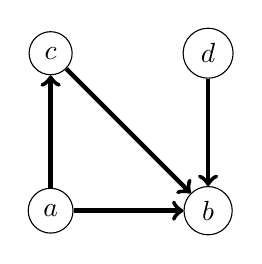
\begin{tikzpicture}
	\node[draw,circle] (a) at (0,0){$a$};
	\node[draw,circle] (b) at (2,0){$b$};
	\node[draw,circle] (c) at (0,2){$c$};
	\node[draw,circle] (d) at (2,2){$d$};
	\draw[ultra thick,->] (a) -- (b);
	\draw[ultra thick,->] (a) -- (c);
	\draw[ultra thick,->] (c) -- (b);
	\draw[ultra thick,->] (d) -- (b);
	\end{tikzpicture}
	\end{enumerate}
	\vfill
\newpage

\item Special Matrices
	\begin{enumerate}
	\item $\textbf{0}=\textbf{0}_{m \times n},$ the zero matrix
	\vfill
	\item an $n \times n$ square matrix $A$ and its main diagonal versus its off-diagonal 
	\vfill
	\item a diagonal matrix $D$ 
	\vfill
	\item $I_n$, the $n \times n$ identity matrix
	\vfill
	\item an upper (lower) triangular matrix $A$ 
	\vfill
	\item a block matrix and its submatrices
	\vfill
	\end{enumerate}
\newpage
$A=\bbm 1&2&3\\4&-5&6 \ebm,  \hfill C= \bbm 3&4\\5&-2\\ \pi& \sqrt{2}\\0&-7 \ebm\hfill D=\bbm 2&1&0\\ 0&3&5 \ebm,  \hfill x=\vecthree 1 2 {-3}, \hfill y= \bbm 3 & 2& {-1} \ebm$
\item Things we can do with matrices
	\begin{enumerate}
	\item transpose
	\vfill
	\item matrix addition
	\vfill
	\item scalar multiplication
	\vfill
	\item These operations are well-behaved.
	\vfill
\newpage
	\item \textbf{matrix-vector multiplication}
	\vfill
	\end{enumerate}
\end{enumerate}
\end{document}